\documentclass{article}
\usepackage[a4paper]{geometry}
\usepackage{parskip}
\usepackage{mathtools}
\usepackage{amsmath, amssymb}
\usepackage{color}
\usepackage{graphicx}
\usepackage{enumerate}
\usepackage[dutch,english]{babel}
\usepackage {bm}
\usepackage{wasysym}
\usepackage{listings}
\usepackage{float}
\usepackage{epstopdf}

%\newcommand{\f}{\(f\)}
%\newcommand{\g}{\(g\)}
\newcommand{\Q}{\mathbb{Q}}
%\newcommand{\Z}{\mathbb{Z}}
%\newcommand{\R}{\mathbb{R}}
%\newcommand{\C}{\mathbb{C}}
%\newcommand{\N}{\mathbb{N}}
\newcommand{\QED}{\hfill\ensuremath{\square}}
\newcommand{\rk}{\text{rk}~}
\newcommand{\Dt}{\Delta t}
\newcommand{\myeq}[2]{\stackrel{\mathclap{\mbox{\normalfont\tiny\sffamily#1}}}{#2}}


\definecolor{codegreen}{rgb}{0,0.6,0}
\definecolor{codegray}{rgb}{0.5,0.5,0.5}
\definecolor{codepurple}{rgb}{0.58,0,0.82}
\definecolor{backcolour}{rgb}{0.95,0.95,0.92}
 
\lstdefinestyle{mystyle}{
    backgroundcolor=\color{backcolour},   
    commentstyle=\color{codegreen},
    keywordstyle=\color{magenta},
    numberstyle=\tiny\color{codegray},
    stringstyle=\color{codepurple},
    basicstyle=\footnotesize,
    breakatwhitespace=false,         
    breaklines=true,                 
    captionpos=b,                    
    keepspaces=true,                 
    numbers=left,                    
    numbersep=5pt,                  
    showspaces=false,                
    showstringspaces=false,
    showtabs=false,                  
    tabsize=2
}
\lstset{style=mystyle}
\title{Numerieke Methoden 1 Practicum Traffic Flow}

\author{Casper Barendrecht \& Stijn Moerman\\ s1693441 \& s1696874}

\date{\today}


\begin{document}
\maketitle

Files zijn een alledaags probleem. In dit modelleren we de dichtheid van auto's tijdens een file op een snelweg. We beperken ons tot een eendimensionale snelweg van lengte \(L\) (geen afslagen of meerdere wegen die samenkomen). We vatten de autodichtheid \(\rho(x,t)\) op als een functie van plaats en tijd, hierbij geeft \(x\in[0,L]\) de plaats op de snelweg weer en \(t\in[0,t_e]\) het tijdstip van meten weer, met\(t_e\) het laatste tijdstip waarop wordt gemeten. Dit is schematisch weergegeven in onderstaand figuur.

\begin{figure}[H]
  \centering
  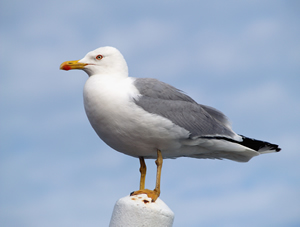
\includegraphics[width=0.5\textwidth]{seagull}
  \caption{Een schematische weergave van een eendimensionaal file probleem}
  \label{fig:bots}
\end{figure}
Dit model is een praktische toepassing van een probleem in de numerieke stromingsleer en is vernoemd naar een Nederlandse natuurkundige Jan Burgers.
Om dit te modelleren, wordt aangenomen dat de autodichtheid op het interval \(x_1,x_2\) enkel kan veranderen door  (MEER UITLEG INLEIDING
\textbf{Opgave 1}\\


Er geldt:
\begin{align}
	\frac{\partial \rho}{\partial t}+\frac{\partial}{\partial x}(\rho(1-\rho))=\nu \frac{\partial^2 \rho}{\partial x^2},~\nu\in \mathbb{R}_+ \label{eq:rho}
	\end{align}
Laten we \(u(x,t)=\alpha\rho + \beta\), dan kan vergelijking \eqref{eq:rho} herschreven worden tot
	\begin{align}
 \frac{\partial u}{\partial t}+\frac{\partial}{\partial x}\left(\frac{1}{2}u^2\right) = \nu \frac{\partial^2 u}{\partial x^2},~\nu\in \mathbb{R}_+\label{eq:u}
\end{align}
Door de afgeleiden van \(u(x,t)\) in termen van \(p(x,t)\) te schrijven als volgt,
\begin{align*}
 \frac{\partial u}{\partial t} &=\alpha\frac{\partial \rho}{\partial t}\\
\frac{\partial}{\partial x}\left(\frac{1}{2}u^2\right)&=\frac{1}{2}\frac{\partial}{\partial x}(\alpha^2\rho^2 +2\alpha\beta\rho+\beta^2)= \frac{\alpha}{2}\frac{\partial}{\partial x}\rho(\alpha\rho+2\beta))\\
\nu \frac{\partial^2 u}{\partial x^2}&=\alpha \nu\frac{\partial^2 \rho}{\partial x^2}
\end{align*}
Kunnen we vergelijking \eqref{eq:u} herschrijven tot:
\begin{align*}
	\alpha\frac{\partial \rho}{\partial t}+\frac{\alpha}{2}\frac{\partial}{\partial x}\rho(\alpha\rho+2\beta))=\alpha \nu\frac{\partial^2 \rho}{\partial x^2}\\
		\frac{\partial \rho}{\partial t}+\frac{\partial}{\partial x}\rho(\beta-(-\frac{\alpha}{2})\rho)=\nu\frac{\partial^2 \rho}{\partial x^2}
\end{align*}
We vinden dat vergelijking   \eqref{eq:u} equivalent is aan \eqref{eq:rho} als \(\beta=1\) en \(\alpha=-2\). We vinden dat \(u(x,t)=1-2\rho(x,t)\).\\
Een probleem in deze vorm heet  een conservatieve vorm. \\

Om dit stelsel te integreren, worden eerst de beginvoorwaarden vastgelegd. We beginnen met het simpelste model, (BLABLABLA toevoegen)


\textbf{Opgave 2:}
We hebben:
\begin{align}
\frac{\partial u}{\partial t} &= \nu \frac{\partial^2 u}{\partial x^2} -\frac{\partial}{\partial x}\left(\frac{1}{2}u^2\right) &\text{ voor } 0<x<L, t>0\\\label{eq:u0}
u(0,t) &= -1 &\text{ voor } t\geq 0\\
\frac{\partial u}{\partial x}(L,t) &= 0 &\text{ voor } t\geq 0\\
u(x,0) &= 0 &\text{ voor } 0<x<L
\end{align}
Om het probleem te kunnen simuleren, discretiseren we het probleem zodanig dat $x_0 = 0$, $x_i= i \Delta x$ en $x_{N+1}=L$, dus $\Delta x = \frac{L}{N+1}$.
In het vervolg geldt $u_i=u(x_i)$.
We schrijven de eerste formule in de vorm voor $\vec{u} = (u_1,\dots,u_{N+1})^\intercal$:
\begin{align*}
\dot{\vec{u}} = \nu K \vec{u} - \vec{f}(\vec{u})+\vec{r}(\vec{u})
\end{align*}
Met behulp van de centrale differentie methode geldt:
\begin{align*}
\frac{\partial^2 u}{\partial x^2}(x_i) &= \frac{u_{i-1}-2u_i+u_{i+1}}{\Delta x^2}\\
\left(\frac{\partial}{\partial x}\left(\frac{1}{2}u^2\right)\right)(x_i) &= \frac{-\frac{1}{2}u_{i-1}^2+\frac{1}{2}u_{i+1}^2}{2\Delta x}
= \frac{-u_{i-1}^2+u_{i+1}^2}{4\Delta x}
\end{align*}
voor $2\leq i\leq N$.
Ook hebben we:
\begin{align*}
\frac{\partial^2 u}{\partial x^2}(x_1) &= \frac{u_{0}-2u_1+u_{2}}{\Delta x^2}
\myeq{\eqref{eq:u0}}{=} \frac{-1-2u_1+u_{2}}{\Delta x^2}
= \frac{u_{2}-2u_1}{\Delta x^2} -\frac{1}{\Delta x^2}\\
\left(\frac{\partial}{\partial x}\left(\frac{1}{2}u^2\right)\right)(x_1) &= \frac{-u_{0}^2+u_{2}^2}{4\Delta x}
= \frac{-1+u_{2}^2}{4\Delta x}
= \frac{u_{2}^2}{4\Delta x}+\frac{-1}{4\Delta x}
\end{align*}
Voor $u_{N+1}$ kunnen we onze beginvoorwaarde verwerken d.m.v. het virtuele punt $x_{N+2}$.
We krijgen dan:
\begin{align*}
0=\dot{u}_{N+1} = \frac{-u_{N}+u_{N+2}}{2\Delta x}
\end{align*}
Dus $u_{N+2}=u_N$.
We hebben dan dus:
\begin{align*}
\frac{\partial^2 u}{\partial x^2}(x_{N+1}) &= \frac{u_{N}-2u_{N+1}+u_{N+2}}{\Delta x^2}
= \frac{u_{N}-2u_{N+1}}{\Delta x^2} +\frac{u_{N}}{\Delta x^2}\\
\left(\frac{\partial}{\partial x}\left(\frac{1}{2}u^2\right)\right)(x_{N+1}) &= \frac{-u_{N}^2+u_{N+2}^2}{4\Delta x}
= \frac{-u_{N}^2}{4\Delta x} +\frac{u_{N}^2}{4\Delta x}
\end{align*}

Dus we krijgen dan:
\begin{align*}
K = \frac{1}{\Delta x^2}\cdot\begin{pmatrix}
-2 & 1 & 0 & \hdots & 0 & 0\\
1 & -2 & 1 & \hdots & 0 & 0\\
0 & 1 & -2 & \hdots & 0 & 0\\
\vdots & \vdots & \vdots & \ddots & \vdots\\
0 & 0 & 0 & \hdots & -2 & 1\\
0 & 0 & 0 & \hdots & 1 & -2\\
\end{pmatrix}
\end{align*}
en
\begin{align*}
\vec{f}(\vec{u}) = \frac{1}{4\Delta x}\cdot
\begin{pmatrix}
u_2^2\\
-u_1^2 + u_3^2\\
\vdots\\
-u_{i-1}^2+u_{i+1}^2\\
\vdots\\
-u_{N-1}^2+u_{N+1}^2\\
-u_N^2\\
\end{pmatrix}
&&
\vec{r}(\vec{u}) = 
\begin{pmatrix}
\frac{-\nu}{\Delta x^2} + \frac{1}{4\Delta x}\\
0\\
\vdots\\
0\\
\frac{\nu u_N}{\Delta x} + \frac{-u_N^2}{4\Delta x}\\
\end{pmatrix}
\end{align*}

\textbf{Opgave 3}
Mooie tabel is mooi:

\begin{table}[H]
\centering
\label{tab:specs}
\begin{tabular}{|l|l|l|l|l|}
\hline
\(v\) & \(N\) & \(L\) & \(t_e\) & \(\Dt\) \\ \hline
 0.5 & 100 & 3.0 & 5.0 & 0.0001 \\ \hline
\end{tabular}
\caption{Startvoorwaarden}
\end{table}

\textbf{Opgave 4}
Om te kijken hoe groot we $\Dt$ kunnen kiezen, schrijven we voor alle $i$:
\begin{align*}
\dot{u}_i =g_i(\vec{u})
\end{align*}
We hebben dan dus (met $2\leq i \leq N$):
\begin{align*}
g_1(\vec{u})&=\dot{u}_1 = \nu \frac{-2u_1+u_2}{\Delta x^2} -\frac{u_2^2}{4\Delta x} -\frac{\nu}{\Delta x^2} +\frac{1}{4\Delta x}\\
g_i(\vec{u})&=\dot{u}_i = \nu \frac{u_{i-1}-2u_i+u_{i+1}}{\Delta x^2} -\frac{-u_{i-1}^2+u_{i+1}^2}{4\Delta x}\\
g_{N+1}(\vec{u})&=\dot{u}_{N+1} = \nu \frac{u_{N}-2u_{N+1}}{\Delta x^2} -\frac{-u_N^2}{4\Delta x} +\frac{\nu u_N}{\Delta x^2} -\frac{u_N^2}{4\Delta x}
=2\nu \frac{u_N}{\Delta x^2} -2\nu\frac{u_{N+1}}{\Delta x^2}
\end{align*}
Voor de stabiliteit willen we nu kijken hoe groot de eigenwaarden van de Jacobi-matrix $J$ van $\vec{g}(\vec{u})$ kunnen zijn.
We vinden (voor $2\leq i\leq N$):
\begin{align*}
J_{1,1} &= \frac{\partial g_1}{\partial u_1} = \frac{-2\nu}{\Delta x^2}\\
J_{1,2} &= \frac{\partial g_1}{\partial u_2} = \frac{\nu}{\Delta x^2} -\frac{u_2}{2\Delta x}\\
J_{i,i-1} &= \frac{\partial g_i}{\partial u_{i-1}} = \frac{\nu}{\Delta x^2}+\frac{u_{i-1}}{2\Delta x}\\
J_{i,i} &= \frac{\partial g_i}{\partial u_i} = \frac{-2\nu}{\Delta x^2}\\
J_{i,i+1} &= \frac{\partial g_i}{\partial u_{i+1}} = \frac{\nu}{\Delta x^2} -\frac{u_{i+1}}{2\Delta x}\\
J_{N+1,N} &= \frac{\partial g_{N+1}}{\partial u_N} =  \frac{2\nu}{\Delta x^2}\\
J_{N+1,N+1} &= \frac{\partial g_{N+1}}{\partial u_{N+1}} = \frac{-2\nu}{\Delta x^2}
\end{align*}
Door in deze Jacobi-matrix de beginvoorwaarde $u(x,0) =0$ in te vullen krijgen we:
\begin{align*}
J(\vec{u}(\vec{x},0)) = \frac{\nu}{\Delta x^2}
\begin{pmatrix}
-2 & 1 & &&\\
1 &\ddots &\ddots&&\\
&\ddots &\ddots&1&\\
& &1&-2&1\\
& &&2&-2\\
\end{pmatrix}
\end{align*}
M.b.v. de methode van Gerschgorin kijken we waar de eigenwaarden van deze matrix moeten liggen.
Deze methode zegt dat elke eigenwaarde $\lambda$ aan minstens een van de volgende eisen moet voldoen:
\begin{align*}
\left|\lambda + \frac{2\nu}{\Delta x^2}\right| \leq \frac{\nu}{\Delta x^2}\\
\left|\lambda + \frac{2\nu}{\Delta x^2}\right| \leq \frac{2\nu}{\Delta x^2}\\
\left|\lambda + \frac{2\nu}{\Delta x^2}\right| \leq \frac{2\nu}{\Delta x^2}
\end{align*}
Dus er geldt:
\begin{align*}
\left|\frac{\Delta x^2}{2\nu} \cdot\lambda +1\right|\leq 1
\end{align*}

Voor de stabiliteit van Euler voorwaarts moet elke eigenwaarde $\lambda$ voldoen aan:
\begin{align*}
\left|\Delta t \cdot\lambda +1\right|\leq 1
\end{align*}
Kortom, voor stabiliteit moet er gelden: $\Delta t \leq \frac{\Delta x^2}{2\nu} =\frac{L^2}{2\nu(N+1)^2}$.
Met de gekozen waarden uit opgave $3$ vinden we een maximale tijdstap van:
\begin{align*}
\Delta t \leq \frac{3^2}{2\cdot 0.5 \cdot(100 +1)^2} = \frac{9}{10201}
\end{align*}

\textbf{Opgave 6}
Laat nu: 
\begin{align*}
	u(x,0) =\begin{cases}
	1, & 0\leq x \leq L/3,\\
	2-(3/L)x, & L/3 \leq x\leq 2L/3,\\
	0, & 2L/3 \leq x
	\end{cases}
\end{align*}
samen met de nieuwe randvoorwaarden 
\begin{align*}
u(0,t)=1,&&\frac{\partial u}{\partial x}(L,t)=0,&&\mbox{voor }t\geq 0
\end{align*}
en de nieuwe parameters:
\begin{table}[H]
\centering
\label{tab:specs2}
\begin{tabular}{|l|l|l|l|l|}
\hline
\(v\) & \(N\) & \(L\) & \(t_e\) & \(\Dt\) \\ \hline
 0.01 & 100 & 3.0 & 5.0 & 0.003 \\ \hline
\end{tabular}
\caption{Startvoorwaarden}
\end{table}

We hebben nu: $u(0,t) = 1$, dus krijgen we:
\begin{align*}
-\frac{\partial^2 u}{\partial x^2}(x_1) &= \frac{-u_{0}+2u_1-u_{2}}{\Delta x^2}
= \frac{-1+2u_1-u_{2}}{\Delta x^2}
= \frac{2u_1-u_{2}}{\Delta x^2} +\frac{-1}{\Delta x^2}
\end{align*}

Voor het opgewonden schema hebben we:
\begin{align*}
\dot{u}_{i} =\frac{-u_{i-1}+u_{i}}{\Delta x}
\end{align*}
Dus hebben we voor $2\leq i \leq N+1$:
\begin{align*}
\left(\frac{\partial}{\partial x}\left(\frac{1}{2}u^2\right)\right)(x_i) &= \frac{-\frac{1}{2}u_{i-1}^2+\frac{1}{2}u_{i}^2}{2\Delta x}
= \frac{-u_{i-1}^2+u_{i}^2}{4\Delta x}
\end{align*}
en verder ook:
\begin{align*}
\left(\frac{\partial}{\partial x}\left(\frac{1}{2}u^2\right)\right)(x_1) &= \frac{-\frac{1}{2}u_{0}^2+\frac{1}{2}u_{1}^2}{2\Delta x}
= \frac{-u_{0}^2+u_{1}^2}{4\Delta x}
=\frac{u_1^2}{4\Delta x} + \frac{-1}{4\Delta x}
\end{align*}
We krijgen dus een nieuwe $\vec{f}$ en $\vec{r}$:
\begin{align*}
\vec{f}(\vec{u}) =
\frac{1}{4\Delta x} \cdot
\begin{pmatrix}
u_1^2\\
-u_1^2 + u_2^2\\
\vdots\\
-u_{i-1}^2+u_{i}^2\\
\vdots\\
-u_{N-1}^2+u_{N}^2\\
-u_N^2+u_{N+1}^2\\
\end{pmatrix}
 &&
\vec{r}(\vec{u}) = 
\begin{pmatrix}
\frac{\nu}{\Delta x^2} + \frac{1}{4\Delta x}\\
0\\
\vdots\\
0\\
\frac{\nu u_N}{\Delta x^2}\\
\end{pmatrix}
\end{align*}

\end{document}
%plaatje opgave 5 is op t=0.3600
